\chapter{Longitudinal Method}

\section{Objectives of Longitudinal Research} 
The five objectives for longitudinal research are: 
    \begin{enumerate}
        \item Direct identification of intraindividual change and stability 
        \item Identification of interindividual differences or similarity 
        \item Analysis of interrelationships in behavioral change 
        \item Aanalysis of causes (determinants) of intraindividual change (determinants are dynamic, very within an individual over time) 
        \item Analysis of causes (determinants) of interindividual differences in intraindividual change (determinants are static, vary only between-individuals) 
    \end{enumerate}





\section{Multilevel / Hierarchical Analysis} 
Designed to account for nested data, also known as hierarchical linear models, mixed-effects models, random-coefficient or random-effects models. 

\subsection{Decomposition of Variance} 
MLM focuses on the decomposition of between cluster variance and within cluster variance, as well as the ratio between cluster variance to total variance (Intra-class Correlation). Cluster-level predictors are used to explain between-cluster variation, and individual-level predictors are used to explain within-cluster variation 

\subsection{Basic Multilevel Equation} 
\begin{align*}
    & y_{ij} = b_{0j} + e_{ij} \\
    & b_{0j} = \beta_{00} + u_{0j}\\
    & e_{ij} \sim N(0, \sigma_e^2) \\
    & u_{0j} \sim N(0, \sigma_{u0}^2)
\end{align*}
\begin{itemize}
    \item $y_{ij}$ Observed score for student $i$ in school $j$
    \item $b_{0j}$ Intercept for school $j$ (School specific mean) 
    \item $e_{ij}$ Deviation for child $i$ in school $j$ w.r.t school $j$ average 
    \item $\beta_{00}$ Grand mean 
    \item $u_{0j}$ Deviation for school $j$ mean w.r.t overall mean
    \item Notice that level 1 variance $\sigma_e^2$ and level 2 variance $\sigma_{u0}^2$ are orthogonal. Together they account for total variance
\end{itemize}

\subsection{Multilevel Equation with level 1 predictor} 
\begin{align*}
    & y_{ij} = b_{0j} + b_{1j}\cdot x_{ij} + e_{ij} \\
    & b_{0j} = \beta_{00} + u_{0j}\\
    & b_{1j} = \beta_{10} + u_{1j}\\
    & e_{ij} \sim N(0, \sigma_e^2) \\
    & u_{0j}, u_{1j} \sim N(
        \begin{bmatrix} 0 \\ 0 \end{bmatrix}, 
        \begin{bmatrix} \sigma_{u0}^2 & \sigma_{u1,u0} \\ \sigma_{u1,u0} & \sigma_{u1}^2 \end{bmatrix} )
\end{align*}
\begin{itemize}
    \item $y_{ij}$ Observed score for student $i$ in school $j$
    \item $b_{0j}$ Intercept for school $j$ (School specific mean) 
    \item $x_{ij}$ Feature $x$ for student $i$ in school $j$ 
    \item $e_{ij}$ Deviation for child $i$ in school $j$ w.r.t school $j$ average 
    \item $\beta_{00}$ Grand mean 
    \item $u_{0j}$ Deviation for school $j$ mean w.r.t overall mean intercept
    \item $u_{1j}$ Deviation of school $j$'s $b_1$ slope w.r.t overall mean
\end{itemize}



\subsection{Multilevel Equation with level 2 predictor} 
\begin{align*}
    & y_{ij} = b_{0j} + e_{ij} \\
    & b_{0j} = \beta_{00} + \beta_{01} \cdot z_j + u_{0j}\\
    & e_{ij} \sim N(0, \sigma_e^2) \\
    & u_{0j} \sim N(0, \sigma_{u0}^2)
\end{align*}
\begin{itemize}
    \item $\beta_{01}$ Slope for observed school level predictor $z$
\end{itemize}

\subsection{Multilevel Equation with both level 1 and 2 predictor} 
\begin{align*}
    & y_{ij} = b_{0j} + b_{1j} \cdot x_{ij} + e_{ij}\\
    & b_{0j} = \beta_{00} + \beta_{01} \cdot z_j + u_{0j} \\
    & b_{1j} = \beta_{10} + \beta_{11} \cdot z_j + u_{1j}
\end{align*}

\subsection{Code Example in R: Empty Model} 
Context: read\_ks is the outcome variable. Students are clustered by school with school id. 
The model is 
    \begin{align*}
        y 
        & = b_{0j} + e_{ij} \\
        & = (\beta_{00} + u_{0j}) + e_{ij}
    \end{align*}
\begin{R}
library(nlme)
# Empty Model - lme 
read.empty.lme = lme(read_ks ~ 1, random = ~1|school_id, data = ecols_school, na.action = "na.omit")

# Equivalent: 
read.empty <- nlme(read_ks ~ beta_00 + u_0j, data = ecl_school, fixed = beta_00~1, random = u_0j~1, group = ~school_id, start = c(beta_00=35), na.action = "na.omit")
\end{R}
    \begin{itemize}
        \item read\_ks ~ 1: outcome is only depends on the intercept 
        \item random = ~1 | school\_id: Intercept is allowed to be different by school
    \end{itemize}


\subsection{Code Example in R: Model with Predictor} 
Context: $read\_ks$ is the outcome variable, $attent\_m$ is the school mean attention, $attent\_d$ is the individual deviation from the school mean. 
The model is 
    \begin{align*}
        y 
        & = b_{0j} + b_{1j} \cdot x_{ij} + e_{ij} \\
        & = (\beta_{00} + \beta_{01} * attent\_m + u_{0j}) + (\beta_{10} + u_{1j}) \cdot attent\_d + e_{ij}
    \end{align*}

\begin{R}
read.attent.lme = lme(read_ks ~ attent_m + attent_d, random = ~attent_d|school_id, data = ecls_school, na.action = na.exclude) 

# Equivalent 

read.attent <- nlme(read_ks ~ (beta_00 + beta_01 * attent_m + u_0j) + (beta_10 + u_1j) * attent_d, 
    data = ecls_school, 
    fixed = beta_00 + beta_01 + beta_10 ~ 1. 
    random = u_0j + u_1j ~ 1, 
    group = ~ school_id, 
    start = c(beta_00 = 35, beta_01 = 0, beta_10 = 0), 
    na.action = na.exclude
\end{R}






\subsection{Code Example in R: Adding another predictor} 
The Model is 
    \begin{align*}
        & y \\
        & = (\beta_{00} + \beta_{01} * attent\_m + \beta_{02} * hrs\_day5 + u_{0j}) \\
        & \qquad + (\beta_{10} + \beta_{11} * hrs\_day5 + u_{1j}) * attent\_d + e_{ij}
    \end{align*}


\begin{R}
# Add another school level predictor 
read.full.lme = lme(read_ks ~ attent_m + attent_d + hrs_day5 + attent_d * hrs_day5, random = ~attent_d | school_id ...)

# Equivalent 
read.full <- nlme(read_ks ~ (beta_00 + beta_01 * attent_m + beta_02 * hrs_day5 + u_0j) + (beta_10 + beta_11 * hrs_day5 + u_1j) * attent_d
\end{R}





\section{Structural Equation Modeling}

\paragraph{High Level Summary}: SEM models the covariance structure exists within the data. Manifest variables are the observed variables defining the structure we wish to model. Latent variables are the unobserved variables implied by the covariance among two or more manifest variables. Following are the common component of the path diagram associated with SEM
    \begin{itemize}
        \item Squares: observed variables
        \item Circles: Latent variables
        \item Double-headed arrows: Variances / Covariances (Association)
        \item Single-headed arrows: Regressions (Direct effect) 
        \item Triangle: Constant (vector of 1) used to modeling means. Note double-headed arrow on a constant doesn't mean variance. It represent mean squared. 
    \end{itemize}
    
\subsection{SEM Demo with a Simple Regression} 
Notice in the  simple regression, variance of $y_i$ is decomposed into variance explained by $x_i(\sigma_x^2 \cdot b_1^2)$ and unexplained variance $(\sigma_e^2)$. The path diagram is figure \ref{fig:sem_path_simp_reg}
    \begin{figure}[ht]
        \centering
        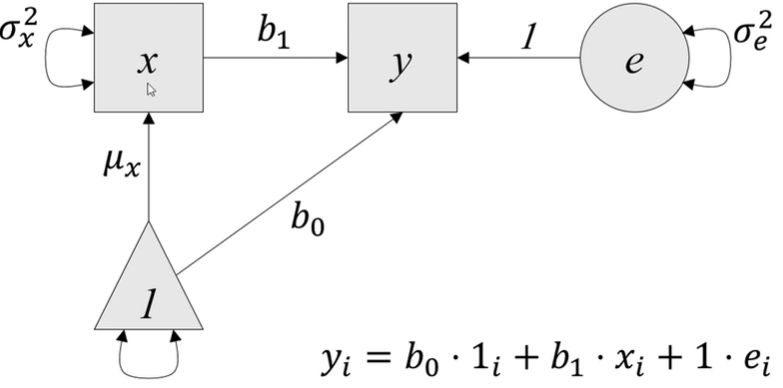
\includegraphics[width = 4cm, height = 3cm]{images/001_sem_simp_reg.png}
        \caption{Path Diagram for Simple Linear Regression}
        \label{fig:sem_path_simp_reg}
    \end{figure}
Some key observation on the path diagram: 
    \begin{itemize}
        \item How 1 specifies both the intercept for $y$, as well as the variance for $x$. 
        \item We can replace the latent variable $e$ with a two headed arrow with $\sigma_e^2$. Notice this two headed arrow doesn't mean variance of $y$. It means the residual variance of $y$. 
        \item The variance of $x$ is given by the two headed arrow with $\sigma_x^2$
    \end{itemize}
Variance and mean calculation (see explaination at next section): 
    \begin{align*}
        & Var(x) = \sigma_x^2\\
        & Var(y) = (b_1 \times \sigma_x^2 \times b_1) + (1 \times \sigma_e^2 \times 1)\\
        & E[xy] = \sigma_x^2 b_1\\
        & E[x]^2 = \mu_x^2 \\
        & E[y]^2 = (b_1 \times \mu_x \times b_0) + (b_0 \times b_0) + (b_0 \times \mu_x \times b_1) + (b_1 \times \mu_x \times \mu_x \times b_1)
    \end{align*}
Also notice we can go from $x$ to $e$, because in regression $x$ and $e$ is independent. 


\subsection{Structural Expectation Calculation with Path Diagram} 

\paragraph{Structural Expectations} can be calculated based on a path diagram or computed algebraically. Note that we can ignore the constant, since it is only used for mean structure. 
    \begin{figure}[ht]
        \centering
        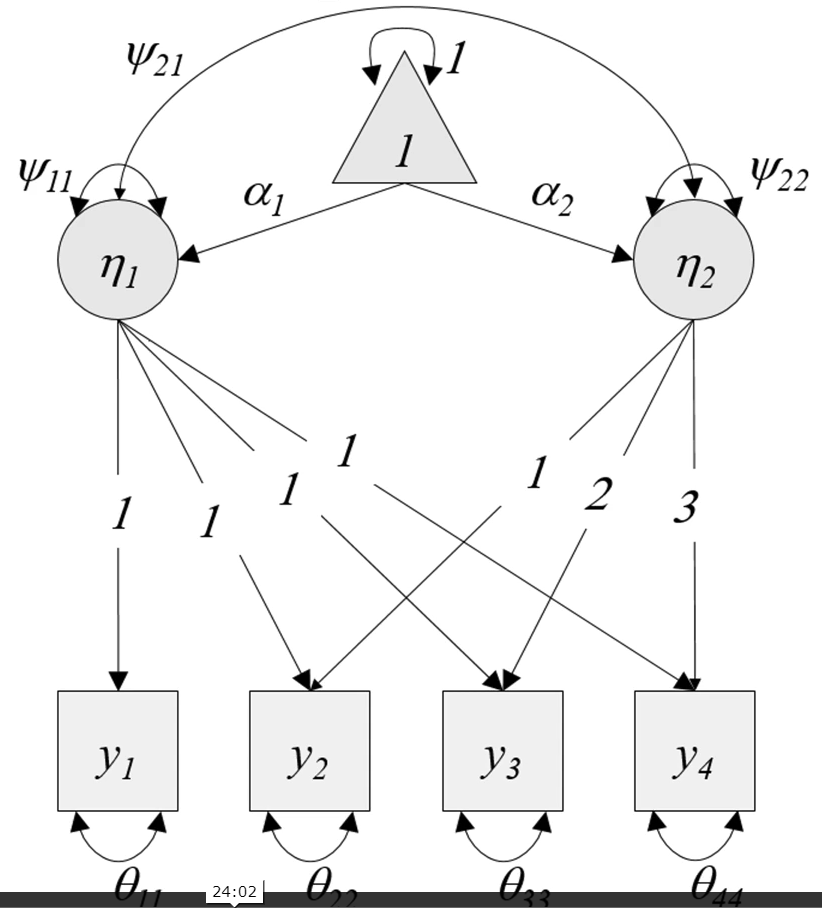
\includegraphics[width = 4cm, height = 6cm]{images/002_sem_expectation_model.png}
        \caption{Path Diagram for Example Model}
        \label{fig:sem_path_expec_mod}
    \end{figure}
To calculate the expected variance of any variable, we need to find all the ways that we can travel to the variable by following the backward, turn (double headed arrow), forward rule. Backward and forward is optional, and can be done multiple times, but turn is required. For example, to calculate variance of $y_1$, we have 
    \begin{itemize}
        \item $y_1$ backward to $\eta_1$, turn at $\eta_1$, and forward to $y_1$. So the variance contribution would be $1 \times \psi_{11} \times 1$
        \item $y_1$ turn to itself. So the variance contribution would be $\theta_{11}$
    \end{itemize}
For $y_2$, we have 5 components
    \begin{itemize}
        \item $y_2$ -> $\eta_1$ (turn to itself)-> $y_2$: $1 \times \psi_{11} \times 1$
        \item $y_2$ -> $\eta_2$ (turn to itself) -> $y_2$: $1 \times \psi_{22} \times 1$
        \item $y_2$ -> $\eta_1$ -> $\eta_2$ -> $y_2$: $1 \times \psi_{21} \times 1$
        \item $y_2$ -> $\eta_2$ -> $\eta_1$ -> $y_2$: $1 \times \psi_{21} \times 1$
        \item $y_2$ turn to itself: $\theta_{22}$
    \end{itemize}
For covariance calculation, we do the same thing by finding all paths that can go from $x$ to $y$. E.g.: For $Cov(y_1, y_2)$ is 
    \begin{align*}
        \left( 1 \times \psi_{11} \times 1\right) + \left(1 \times \psi_{21} \times 1 \right)
    \end{align*}
For mean expectation, we can only turn through the constant variable. E.g.: 
    \begin{align*}
        & y_1 \text{Path: } y_1 \to \eta_1 \to 1 \to \eta_1 \to y_1 \\
        & E[y_1]^2 = 1 \times 1 \times \alpha_1 \times 1 \times \alpha_1 \times 1 \\
        & E[y_2]^2 = \alpha_1^2 + \alpha_2^2 + 2\alpha_1\alpha_2
    \end{align*}
    
\subsection{Structural Expectation Calculation with RAM} 
Three matrices can be used to describe the model
    \begin{itemize}
        \item $A$: Asymmetric Relationships with columns as predictor and rows as outcome
        \item $S$: Symmetric relationships 
        \item $F$: Filter, describe differences between observed (constant counts) and unobserved variables 
    \end{itemize}
Expectations using Ram Notation: 
    \begin{align*}
        & \text{Linear Model:} \qquad v = vA + u \qquad \text{$v$ contains all variables} \\
        & \text{Stochastic expectation} \qquad E[uu'] = S \\
        & \text{Effects Matrix} \qquad E = (I-A)^{-1} \\
        & \text{Expected variance + mean squared matrix} \qquad E[vv'] = ESE'\\
        & \text{for observed variables} \qquad E[v_{obs}v'_{obs}] =  FESE'F'
    \end{align*}

\paragraph{Detail Demo with Regression Model} 
Now consider the simple regression in figure \ref{fig:sem_path_simp_reg}, now with the constant variable named $k$. 
    \begin{align*}
        & F: \text{\# observed variables} \times \text{\# total variables (observed first)} = 3 \times 4\\
        & F = \begin{matrix}
              &   & x & y & k & e & |\\
            x & | & 1 & 0 & 0 & 0 & |\\
            y & | & 0 & 1 & 0 & 0 & |\\
            k & | & 0 & 0 & 1 & 0 & |\\
        \end{matrix} \\
        & A: \text{\# of total variables} \times \text{\# of total variables} = 4 \times 4\\
        & A = \begin{matrix}
              &   & x & y & k & e & | \\
            x & | & 0 & 0 & \mu_x & 0 & |\\
            y & | & b_1 & 0 & b_0 & 1 & |\\
            k & | & 0 & 0 & 0 & 0 & |\\
            e & | & 0 & 0 & 0 & 0 & |\\
        \end{matrix}\\
        & S: Symmetric, \text{\# of total variables} \times \text{\# of total variables} = 4 \times 4\\
        & S = \begin{matrix}
              &   & x & y & k & e & | \\
            x & | & \sigma_x^2 & 0 & 0 & 0 & |\\
            y & | & 0 & 0 & 0 & 0 & |\\
            k & | & 0 & 0 & 1 & 0 & |\\
            e & | & 0 & 0 & 0 & \sigma_e^2 & |\\
        \end{matrix}
    \end{align*}

For actual calculation, we have: 
\begin{align*}
    E 
    & = \left(
        \begin{bmatrix}
            1 & 0 & 0 & 0 \\
            0 & 1 & 0 & 0 \\
            0 & 0 & 1 & 0 \\
            0 & 0 & 0 & 1
        \end{bmatrix}
        - 
            \begin{bmatrix}
            0 & 0 & \mu_x & 0\\
            b_1 & 0 & b_0 & 1\\
            0 & 0 & 0 & 0\\
            0 & 0 & 0 & 0
        \end{bmatrix}
        \right)^{-1}\\
    & = 
        \begin{bmatrix}
            1 & 0 & -\mu_x & 0 \\
            -b_1 & 1 & -b_0 & -1 \\
            0 & 0 & 1 & 0 \\
            0 & 0 & 0 & 1
        \end{bmatrix}^{-1} \\
    & = 
        \begin{bmatrix}
              & x & y & k & e \\
            x & 1 & 0 & \mu_x & 0 \\
            y & b_1 & 1 & b_0 + b_1\mu_x & 1 \\
            k & 0 & 0 & 1 & 0 \\
            e & 0 & 0 & 0 & 1
        \end{bmatrix}\\
\end{align*}
Looking at effect matrix, the column header is the source of effect, and row is the one being affected. So
    \begin{itemize}
        \item The effect of $x$ on $y$ is $b_1$
        \item The expectation of mean of $x$ is $\mu_x$
        \item The mean expectation of $y$ is $b_0 + b_1\mu_x$
    \end{itemize}
Now looking at the sum of squares matrix 
    \begin{align*}
        E[vv'] = 
            \begin{bmatrix}
                \sigma_x^2 + \mu_x^2 &  b_1\sigma_x^2 + \mu_x(b_0 + b_1\mu_x) & \mu_x & 0 \\
                b_1\sigma_x^2 + \mu_x(b_0 + b_1\mu_x) & b_1^2\sigma_x^2 + (b_0 + b_1\mu_x)^2 + \sigma_e^2 & b_0 + b_1\mu_x & \sigma_e^2 \\
                \mu_x & b_0 + b_1\mu_x & 1 & 0 \\
                0 & \sigma_e^2 & 0 & \sigma_e^2
            \end{bmatrix}
    \end{align*}
    \begin{itemize}
        \item Expected variance + mean squares for $x$ is $\sigma_x^2 + \mu_x^2$
        \item Expected variance + mean squares for $y$ is $b_1^2\sigma_x^2 + (b_0 + b_1\mu_x)^2 + \sigma_e^2$
        \item On the off diagonal, if we take all of scores on $x$ and $y$, then taking it average. So it is the expected covariance + expected cross product. 
    \end{itemize}

\subsection{SEM Code Demo} 
    \begin{figure}[ht]
        \centering
        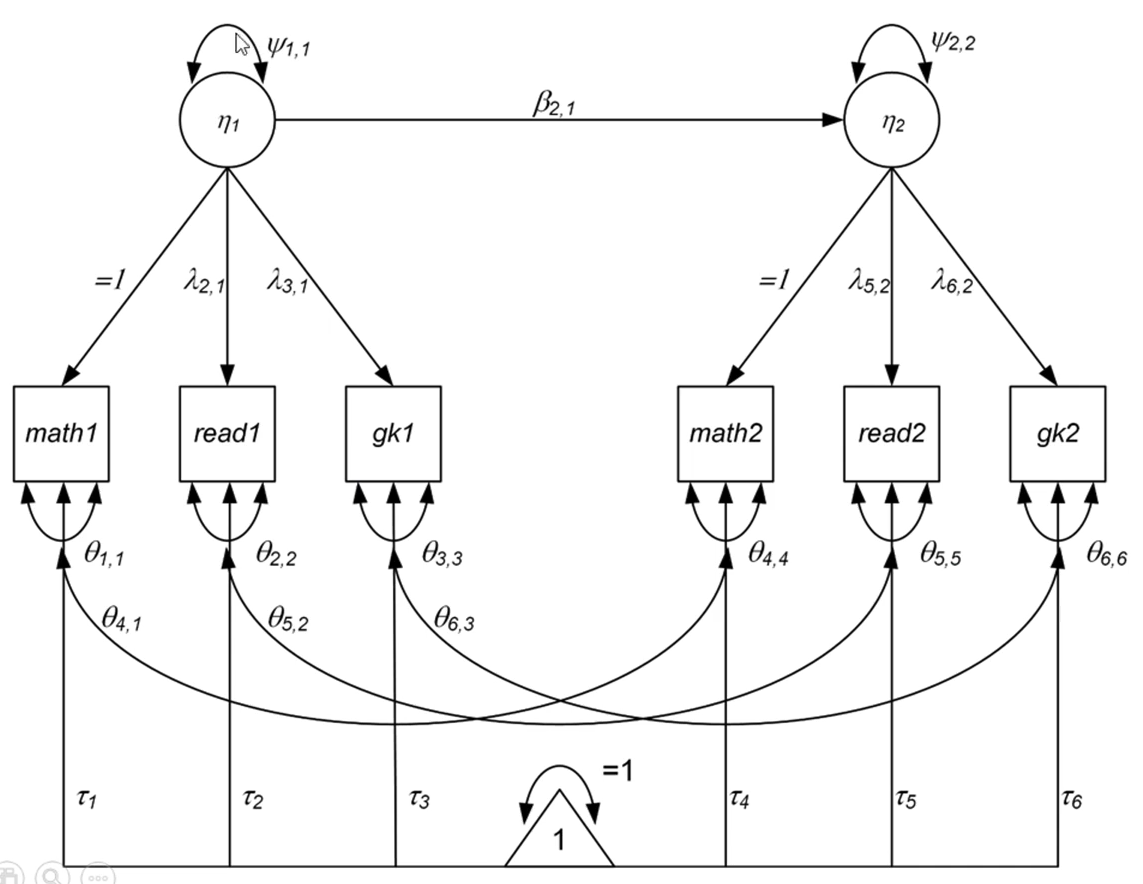
\includegraphics[width = 12cm, height = 9cm]{images/003_sem_program_mod_sample.png}
        \caption{Model Path Diagram}
        \label{fig:sem_program_mod}
    \end{figure}
    
\begin{R}
library(lavaan)
acad.lv = '
    # Factor loading 
    eta_1 = ~ 1*math1 + read1 + gk1
    eta_1 = ~ 1*math2 + read2 + gk2
    
    # Latent variable variances (Psi) 
    eta_1 ~~ eta_1
    eta_2 ~~ eta_2 
    
    # Unique variance (Theta)
    read1 ~~ read1
    math1 ~~ math1
    gk1 ~~ gk1
    
    read2 ~~ read2
    math2 ~~ math2
    gk2 ~~ gk2 
    
    # Unique Covariances (Theta) 
    read1 ~~ read2 
    math1 ~~ math2
    gk1 ~~ gk2
    
    # Latent variable regression (beta) 
    eta_2 ~ start(.8)*eta_1
    
    # Measurement intercepts (nu)
    read1 ~ 1
    math1 ~ 1
    gk1 ~ 1
    
    read2 ~ 1
    math2 ~ 1
    gk2 ~ 1
'

acad.lv.res = lavaan(acad.lv, data = ecls_acad)
summary(acad.lv.res, fit.measure = TRUE)
\end{R}




\section{Growth Model} 


\subsection{No Growth or Intercept Only Model} 
Common and logical starting point for any study of change. Predicts that score do not change over time. So one latent variable (SEM framework) or random coefficient (MLM framework)


\subsubsection{MLM Framework} 
The no growth models in MLM framework are defined as follows: 
    \begin{align*}
        & \text{Level 1 Equation: } y_{ti} = b_{1i} + u_{ti} \\
        & \text{Level 2 Equation: } b_{1i} = \beta_1 + d_{1i} \\
        & \text{Combined view: } y_{ti}= (\beta_1 + d_{1i}) + u_{ti} \\
    \end{align*}
\begin{itemize}
    \item $y_{ti}$ repeatedly observed score at time $t$ for individual $i$ 
    \item $b_{1i}$ random intercept 
    \item $u_{ti}$ time specific residual score. Assumed to follow a normal distribution with mean 0 and constant variance $\sigma_u^2$. The variance is the residual variance, means magnitude of individual variability not captured by the no growth model. 
    \item $\beta_1$ mean for the random intercept 
    \item $d_{1i}$ Individual deviations from the sample mean random intercept, assume to also have a normal distribution with mean 0 and constant variance $\sigma_1^2$. The variance means magnitude of between-person differences in the predicted score over time. 
    \item The three estimates are $\beta_1, \sigma_1^2, \sigma_u^2$
    \item Notice no time included in the model. So no change in scores. 
\end{itemize}

\subsubsection{MLM Code Example} 
Using nlme:nlme(). Assume math is the outcome variable, grade is the time variable, id are clustering variable. 
\begin{R}
#fitting no growth model and assigning it to an object
ng_math_nlme <- nlme(math ~ beta_1 + d_1i,    #model equation
                     data=nlsy_math_long,     #data set                   
                     fixed=beta_1~1,          #fixed parameters              
                     random=d_1i~1,           #random coefficients
                     group=~id,               #clustering variable         
                     start=c(beta_1=40),      #starting values
                     na.action = na.exclude)  #missing data treatment                     

#obtaining summary of the model using the object we just created                     
summary(ng_math_nlme)

\end{R}


\subsubsection{SEM Code Example} 
Using lavaan for SEM and semPlot for ploting the diagram. The dataset are now wide. id is the clustering variable, math2 to math8 are the outcome variable. 
\begin{R}
#writing out no growth model in full SEM way 
ng_math_lavaan_model <- ' 
  # latent variable definitions
      #intercept
      eta_1 =~ 1*math2  # =~ means eta_1 is indicated by factor loading of 1 to math2
      eta_1 =~ 1*math3
      eta_1 =~ 1*math4
      eta_1 =~ 1*math5
      eta_1 =~ 1*math6
      eta_1 =~ 1*math7
      eta_1 =~ 1*math8

  # factor variances
      eta_1 ~~ eta_1 # ~~ means the two headed arrow 

  # covariances among factors 
      #none (only 1 factor)

  # factor means 
      eta_1 ~ start(30)*1 # from triangle to eta_1 

  # manifest variances (made equivalent by naming theta)
      math2 ~~ theta*math2 # two headed arrow for each repeated measured math score 
      math3 ~~ theta*math3
      math4 ~~ theta*math4
      math5 ~~ theta*math5
      math6 ~~ theta*math6
      math7 ~~ theta*math7
      math8 ~~ theta*math8
  # manifest means (fixed at zero)
      math2 ~ 0*1
      math3 ~ 0*1
      math4 ~ 0*1
      math5 ~ 0*1
      math6 ~ 0*1
      math7 ~ 0*1
      math8 ~ 0*1
' #end of model definition

#estimating the model using sem() function
ng_math_lavaan_fit <- sem(ng_math_lavaan_model, 
                          data = nlsy_math_wide,
                          meanstructure = TRUE,
                          estimator = "ML",
                          missing = "fiml")
#diagram of fitted model
semPaths(ng_math_lavaan_fit,what = "path", whatLabels = "par")

#obtaining predicted factor scores for individuals
nlsy_math_predicted <- as.data.frame(cbind(nlsy_math_wide\$id,lavPredict(ng_math_lavaan_fit)))

#naming columns
names(nlsy_math_predicted) <- c("id", "eta_1")

#looking at data
head(nlsy_math_predicted) 

#calculating implied manifest scores
nlsy_math_predicted$math2 <- 1*nlsy_math_predicted$eta_1
nlsy_math_predicted$math3 <- 1*nlsy_math_predicted$eta_1
nlsy_math_predicted$math4 <- 1*nlsy_math_predicted$eta_1
nlsy_math_predicted$math5 <- 1*nlsy_math_predicted$eta_1
nlsy_math_predicted$math6 <- 1*nlsy_math_predicted$eta_1
nlsy_math_predicted$math7 <- 1*nlsy_math_predicted$eta_1
nlsy_math_predicted$math8 <- 1*nlsy_math_predicted$eta_1

\end{R}

The corresponding path diagram is 
\begin{figure}[ht]
    \centering
    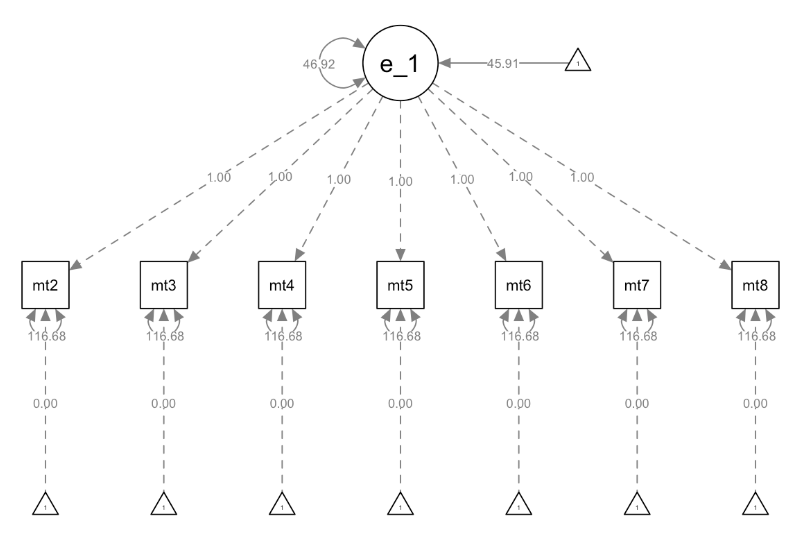
\includegraphics{images/005_no_growth_model_path.png}
    \caption{SEM Path Diagram for No Grwoth Model}
    \label{fig:sem_no_growth_path}
\end{figure}


\subsection{Linear Growth Model} 
Rate of change is constant within an individual, but allowed to vary over individuals. So two latent variables or random coefficients: 
    \begin{itemize}
        \item Intercept: Predicted value at a specific point in time 
        \item Lienar Slope: Predicted rate of change over the observation period 
    \end{itemize}

\subsubsection{MLM Framework} 
The linear growth models in MLM framework are defined as follows: 
    \begin{align*}
        & \text{Level 1 Equation: } y_{ti} = b_{1i} + b_{2i} \cdot \left( \frac{t-k_1}{k_2} \right) + u_{ti} \\
        & \text{Level 2 Equation: } b_{1i} = \beta_1 + d_{1i}, b_{2i} = \beta_2 + d_{2i}\\
        & \text{Combined view: } y_{ti}= (\beta_1 + d_{1i}) + (\beta_2 + d_{2i})  \cdot \left( \frac{t-k_1}{k_2} \right) +  u_{ti}
    \end{align*}
\begin{itemize}
    \item $y_{ti}$ repeatedly observed score at time $t$ for individual $i$ 
    \item $b_{1i}$ random intercept; predicted score for individual $i$ when $t = k_1$
    \item $b_{2i}$ random slope; rate of change for individual $i$ for a one-unit change in $\frac{t}{k_2}$
    \item $t$ time metric, centered and scaled by $k_1, k_2$
    \item $u_{ti}$ time specific residual score. $N(0, \sigma_u^2)$
    \item $\beta_1, \beta_2$ are the mean for the random intercept and slope 
    \item $d_{1i}, d_{2i}$ are individual deviations from their respective sample-level mean. Normally $d_{1i}, d_{2i} \sim N\left(\begin{bmatrix} 0 \\ 0 \end{bmatrix}, \begin{bmatrix} \sigma_1^2 & \sigma_{21} \\ \sigma_{21}^2 & \sigma_2^2 \end{bmatrix} \right) $
    \item The estimates are $\beta_1, \beta_2,  \sigma_1^2, \sigma_2^2, \sigma_{21}, \sigma_u^2$. 
    \item Notice that $\sigma_{21}$ is the covariance between the random intercept and slope, i.e.: degree to which individual deviations in the intercept and slope are linearly associated. (rich get richer effect vs. poor get helped effect). 
    \item Whether $\beta_2 = 0$ means does change exist over time, but $\sigma_2^2$ is also important, since it indicates how much individual differences in $\beta_2$. 
\end{itemize}

\subsubsection{MLM Code Example}
Using nlme:nlme().  Assume math is the outcome variable, grade is the time variable, id are clustering variable.
\begin{R}
#fitting linear growth model and assigning it to an object
lg_math_nlme <- nlme(math~(beta_1+d_1i)+(beta_2+d_2i)*(grade-2),  
                   data=nlsy_math_long,                      
                   fixed=beta_1+beta_2~1,                      
                   random=d_1i+d_2i~1,
                   group=~id,                     
                   start=c(beta_1=35,beta_2=4),
                   na.action = na.exclude)

#obtaining summary of the model using the object we just created
summary(lg_math_nlme)
\end{R}

Using lme, nlme() and lmer function in lme4. Assume math is the outcome variable, grade is the time variable, id are clustering variable.
\begin{R}
#fitting no growth model and assigning it to an object
lg_math_lme <- nlme::lme(math ~ 1 + grade_c2, 
                         random= ~1 + grade_c2|id, 
                         data = nlsy_math_long,
                         na.action = na.exclude,
                         method="ML")


#Alternative way of using nlme 
lg2_math_nlme <- nlme::nlme(math~b_1i+b_2i*(grade-2),
                            data=nlsy_math_long,
                            fixed=b_1i+b_2i~1,
                            random=b_1i+b_2i~1|id,
                            start=c(b_1i=35, b_2i=4),
                            na.action = na.exclude)


# Using lmer
lg_math_lmer <- lme4::lmer(math ~ 1 + grade_c2 + (1 + grade_c2 | id), 
                           data = nlsy_math_long, 
                           REML = TRUE,
                           na.action = na.exclude)
\end{R}


\subsubsection{SEM Framework: Growth models as a Common Factor Model} 
Growth model is modeled as a restricted common factor models with latent variables for the random intercept and slope. The equation is given as 
    \begin{align*}
        & y_i = \Lambda \eta_{i} + u_i\\
        & \eta_{i} = \alpha + \xi_i
    \end{align*}
    \begin{itemize}
        \item $y_i$ is a $T \times 1$ vector of the repeatedly measured observed scores for individual $i$. $T$ is the number of observations across time. 
        \item $\Lambda$ is a $T \times R$ matrix of factor loadings defining the latent growth factors. $R$ is the number of growth factors, $R=1$ means no growth model, and $R=2$ means linear growth models. 
            \begin{itemize}
                \item No growth: $\Lambda = \begin{bmatrix} 1 \\ 1 \end{bmatrix}$ (assuming only two observations) 
                \item Linear growth: $\Lambda = \begin{bmatrix} 1 & \frac{t_1-k_1}{k_2} \\ 1 & \frac{t_2 - k_1}{k_2} \end{bmatrix}$
            \end{itemize}
        \item $\eta_i$ is a $R \times 1$ vector of latent factor scores for individual $i$ 
        \item $u_i$ is a $T \times 1$ vector of residual or unique scores for individual $i$
        \item $\alpha$ is a $R \times 1$ vector of latent factor means 
        \item $\xi_i$ is a $R \times 1$ vector of mean deviations for individual $i$ 
    \end{itemize}
The model expectations for the growth model are 
    \begin{align*}
        & \mu = \Lambda \alpha \\
        & \Sigma = \Lambda \Psi \Lambda^T + \Theta
    \end{align*}
    \begin{itemize}
        \item $\Psi$ is a $R \times R$ latent covariance matrix 
        \item $\Theta$ is a $T \times T$ residual diagonal covariance matrix. We often force the diagonal element of $\Theta$ to be equal, and $\Theta$ to be diagonal. This enforces the assumptions residual is uncorrelated with time. 
    \end{itemize}
Path diagram is given by figure \ref{fig:linear_growth_mod_path_exp}:  
    \begin{figure}[ht]
        \centering
        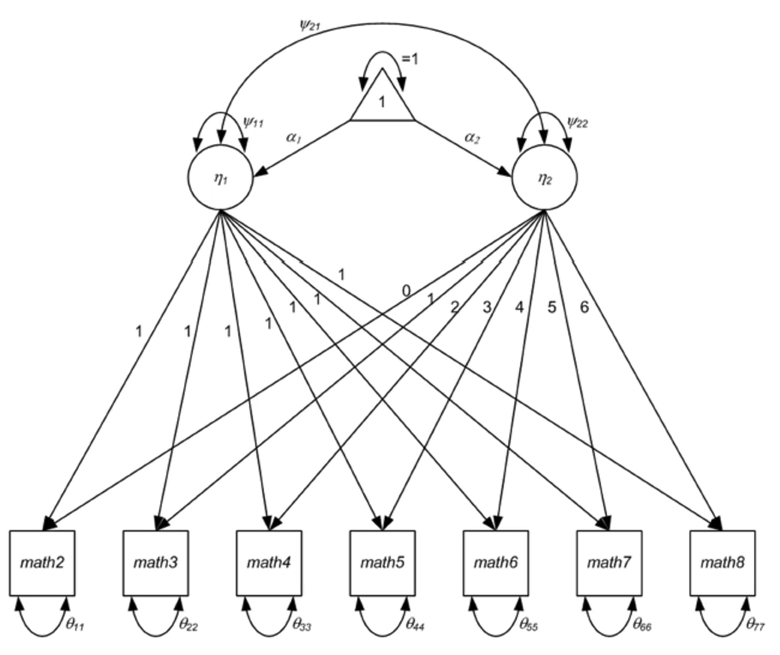
\includegraphics{images/004_linear_growth_model_path.png}
        \caption{Path Diagram for Linear Growth Model with 7 observation}
        \label{fig:linear_growth_mod_path_exp}
    \end{figure}
    \begin{itemize}
        \item $math2$ to $math8$ are the 7 observations 
        \item $\eta_1$ latent variable is the intercept. Hence factor loading is 1 
        \item $\eta_2$ latent variable is the slope, hence factor loading scales linearly with time (0,1,...6) for the 7 math scores. 
        \item $\psi_{11}, \psi_{22}$ are the between person variances on intercept and slope. $\psi_{21}$ is the covariance 
        \item $\alpha_1, \alpha_2$ are the means for intercept and slope. 
        \item $\theta_{11}$ to $\theta_{77}$ are the diagonal entry of the matrix $\Theta$ or the residual variance of each observation. Generally enforced to be the same. 
    \end{itemize}
Mapping between SEM and MLM: 
    \begin{itemize}
        \item $\eta_i$ vector == $b_{1i}$ and $b_{2i}$
        \item $\Lambda$ matrix == functional relationship between the latent variables and the repeatedly measured scores. We don't see this explicitly in the MLM model, but the linear addition in MLM is mapped to this matrix operation
        \item $u_i$ vector == $u_{ti}$ 
        \item $\alpha$ vector == $\beta_1, \beta_2$ 
        \item $\xi_i$ vector == $d_{1i}, d_{2i}$ 
        \item $\Psi$ matrix == $\sigma_1^2$ in the no growth model, and the covariance matrix in the linear growth model. 
        \item $\Theta$ matrix == $\begin{bmatrix}\sigma_u^2 & & \\ & \ddots & \\ &&\sigma_u^2 \end{bmatrix}$
    \end{itemize}

\subsubsection{SEM Code Example} 
Using lavaan for SEM and semPlot for ploting the diagram. The dataset are now wide. id is the clustering variable, math2 to math8 are the outcome variable. 

\begin{R}
#writing out linear growth model in full SEM way 
lg_math_lavaan_model <- '
  # latent variable definitions
      #intercept (note intercept is a reserved term)
      eta_1 =~ 1*math2
      eta_1 =~ 1*math3
      eta_1 =~ 1*math4
      eta_1 =~ 1*math5
      eta_1 =~ 1*math6
      eta_1 =~ 1*math7
      eta_1 =~ 1*math8

      #linear slope 
      eta_2 =~ 0*math2
      eta_2 =~ 1*math3
      eta_2 =~ 2*math4
      eta_2 =~ 3*math5
      eta_2 =~ 4*math6
      eta_2 =~ 5*math7
      eta_2 =~ 6*math8

  # factor variances
      eta_1 ~~ eta_1
      eta_2 ~~ eta_2

  # covariances among factors 
      eta_1 ~~ eta_2

  # factor means 
      eta_1 ~ start(35)*1
      eta_2 ~ start(4)*1

  # manifest variances (made equivalent by naming theta)
      math2 ~~ theta*math2
      math3 ~~ theta*math3
      math4 ~~ theta*math4
      math5 ~~ theta*math5
      math6 ~~ theta*math6
      math7 ~~ theta*math7
      math8 ~~ theta*math8
  # manifest means (fixed at zero)
      math2 ~ 0*1
      math3 ~ 0*1
      math4 ~ 0*1
      math5 ~ 0*1
      math6 ~ 0*1
      math7 ~ 0*1
      math8 ~ 0*1
' #end of model definition

#obtaining predicted factor scores for individuals
nlsy_math_predicted <- as.data.frame(cbind(nlsy_math_wide\$id,lavPredict(lg_math_lavaan_fit)))

#naming columns
names(nlsy_math_predicted) <- c("id", "eta_1", "eta_2")

head(nlsy_math_predicted)

#calculating implied manifest scores
nlsy_math_predicted$math2 <- 1*nlsy_math_predicted$eta_1 + 0*nlsy_math_predicted$eta_2
nlsy_math_predicted$math3 <- 1*nlsy_math_predicted$eta_1 + 1*nlsy_math_predicted$eta_2
nlsy_math_predicted$math4 <- 1*nlsy_math_predicted$eta_1 + 2*nlsy_math_predicted$eta_2
nlsy_math_predicted$math5 <- 1*nlsy_math_predicted$eta_1 + 3*nlsy_math_predicted$eta_2
nlsy_math_predicted$math6 <- 1*nlsy_math_predicted$eta_1 + 4*nlsy_math_predicted$eta_2
nlsy_math_predicted$math7 <- 1*nlsy_math_predicted$eta_1 + 5*nlsy_math_predicted$eta_2
nlsy_math_predicted$math8 <- 1*nlsy_math_predicted$eta_1 + 6*nlsy_math_predicted$eta_2

#reshaping wide to long
nlsy_math_predicted_long <- reshape(data=nlsy_math_predicted, 
                          timevar=c("grade"), 
                          idvar="id",
                          varying=c("math2", "math3", "math4", 
                                    "math5", "math6", "math7", "math8"),
                          direction="long", sep="")

\end{R}
The diagram is given as 
\begin{figure}[ht]
    \centering
    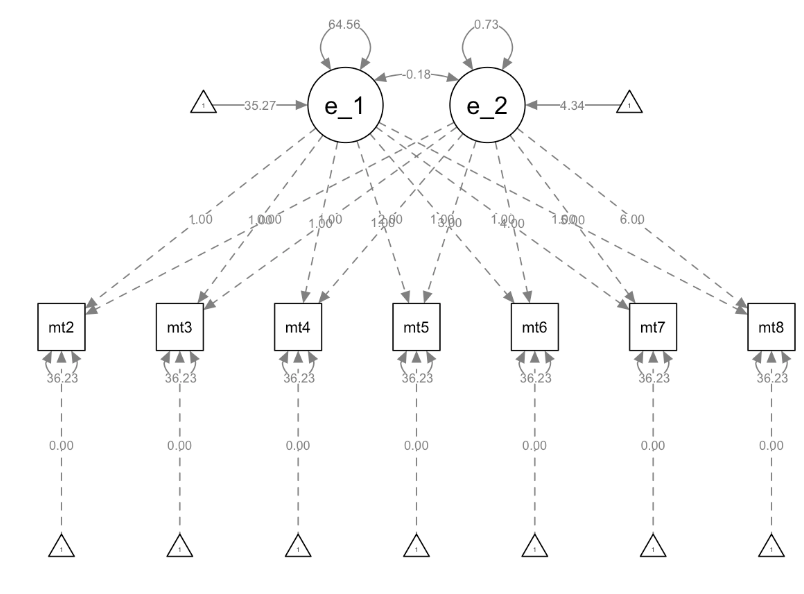
\includegraphics{images/006_linear_growth_model_path.png}
    \caption{Model Path Diagram (Note same as example diagram above}
    \label{fig:linear_growth_mod_path}
\end{figure}